\begin{frame}
  \frametitle{Description générale du dispositif}
  \framesubtitle{Les composants moniteur et contrôleur}
  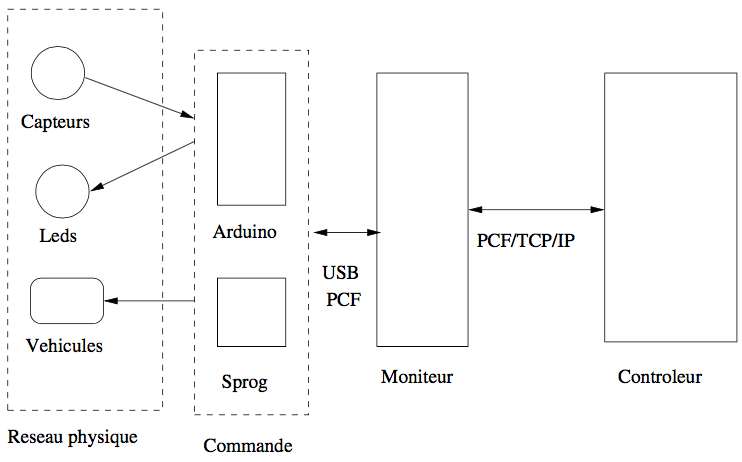
\includegraphics[scale=0.45]{include/communication.png}
\end{frame}

%----------------------------------------------------

\begin{frame}
  \frametitle{Objectifs}
  Placé dans le cadre de la spécification fournie par nos encadrants, ce projet STL
  a pour objectifs :
  \vspace{1em}
  \begin{enumerate}
  \item Conception d'un système de communication contrôleur/moniteur
    \vspace{1em}
  \item Conception d'un système de gestion des règles de circulation
    \vspace{1em}
  \item Implémentation d'une interface graphique
    \vspace{1em}
  \item Tester le contrôleur sur un circuit réel
  \end{enumerate}
\end{frame}

\begin{frame}
  \frametitle{Organisation}
  Nous pouvons présenter l'organisation de ce projet, en développant les trois points suivant :
  \vspace{1em}
  \begin{itemize}
  \item Travail collaboratif
    \vspace{1em}
  \item Planning
    \vspace{1em}
  \item Réunions
  \end{itemize}
\end{frame}

